\documentclass[tikz,border=2pt]{standalone}
\usepackage{amsmath,amssymb}
\usepackage{pgfplots}
\pgfplotsset{compat=1.18}
\usetikzlibrary{calc}

\begin{document}
% Level curves of x^T A x for the four kinds of definiteness: ellipses (bowl, positive
% definite), ellipses with negative values (cap, negative definite), parallel lines
% (semidefinite: a direction with x^T A x = 0), hyperbolas (indefinite: both signs).
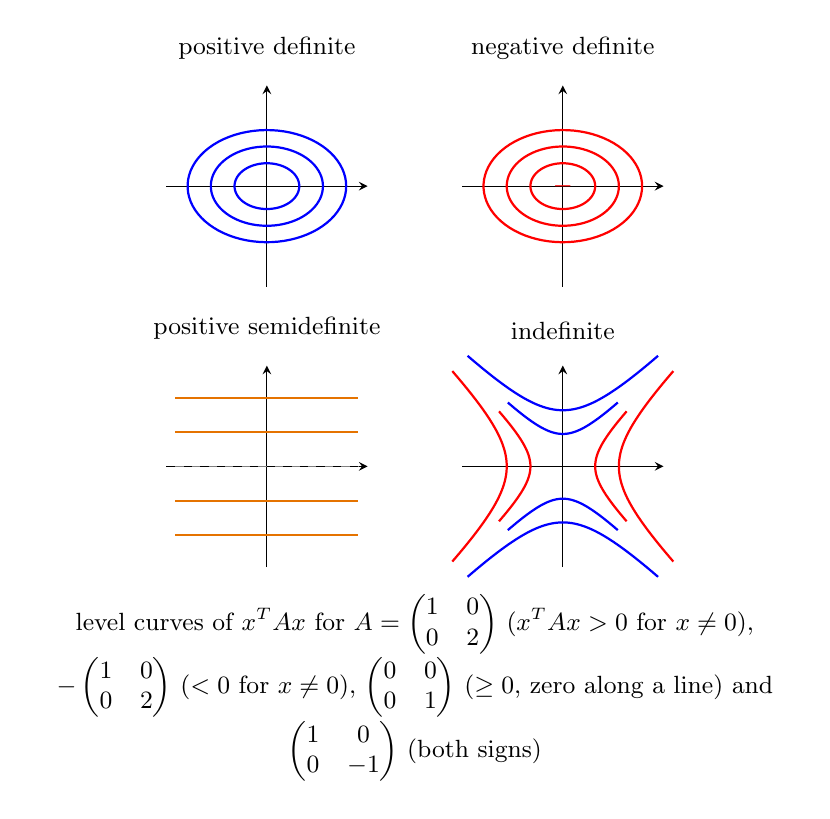
\begin{tikzpicture}
	\begin{axis}[name=p1, axis lines=middle, axis equal image, xmin=-2.2, xmax=2.2, ymin=-2.2, ymax=2.2, xtick=\empty, ytick=\empty, clip=false, width=4.8cm, title={positive definite}, title style={font=\small}]
		\foreach \c in {0.5,1.5,3} {\addplot[blue, thick, domain=0:360, samples=80] ({sqrt(\c)*cos(x)}, {sqrt(\c/2)*sin(x)});}
	\end{axis}
	\begin{axis}[name=p2, at={(p1.east)}, anchor=west, xshift=1.2cm, axis lines=middle, axis equal image, xmin=-2.2, xmax=2.2, ymin=-2.2, ymax=2.2, xtick=\empty, ytick=\empty, clip=false, width=4.8cm, title={negative definite}, title style={font=\small}]
		\foreach \c in {0.5,1.5,3} {\addplot[red, thick, domain=0:360, samples=80] ({sqrt(\c)*cos(x)}, {sqrt(\c/2)*sin(x)});}
		\node[red, font=\small] at (axis cs:0,0) {$-$};
	\end{axis}
	\begin{axis}[name=p3, at={(p1.south)}, anchor=north, yshift=-1.0cm, axis lines=middle, axis equal image, xmin=-2.2, xmax=2.2, ymin=-2.2, ymax=2.2, xtick=\empty, ytick=\empty, clip=false, width=4.8cm, title={positive semidefinite}, title style={font=\small}]
		\foreach \c in {-1.5,-0.75,0.75,1.5} {\addplot[orange!90!black, thick, domain=-2:2, samples=2] ({x}, {\c});}
		\addplot[gray, dashed, domain=-2:2, samples=2] ({x}, {0});
	\end{axis}
	\begin{axis}[name=p4, at={(p3.east)}, anchor=west, xshift=1.2cm, axis lines=middle, axis equal image, xmin=-2.2, xmax=2.2, ymin=-2.2, ymax=2.2, xtick=\empty, ytick=\empty, clip=false, width=4.8cm, title={indefinite}, title style={font=\small}]
		\foreach \c in {0.5,1.5} {
			\addplot[red, thick, domain=-1.3:1.3, samples=60] ({sqrt(\c)*cosh(x)}, {sqrt(\c)*sinh(x)});
			\addplot[red, thick, domain=-1.3:1.3, samples=60] ({-sqrt(\c)*cosh(x)}, {sqrt(\c)*sinh(x)});
			\addplot[blue, thick, domain=-1.3:1.3, samples=60] ({sqrt(\c)*sinh(x)}, {sqrt(\c)*cosh(x)});
			\addplot[blue, thick, domain=-1.3:1.3, samples=60] ({sqrt(\c)*sinh(x)}, {-sqrt(\c)*cosh(x)});
		}
	\end{axis}
	\node[anchor=north, align=flush center, text width=9.6cm, font=\small, yshift=-6pt] at ($(p3.south)!0.5!(p4.south)$) {level curves of $x^{T}Ax$ for $A=\begin{pmatrix}1&0\\0&2\end{pmatrix}$ ($x^{T}Ax>0$ for $x\neq0$), $-\begin{pmatrix}1&0\\0&2\end{pmatrix}$ ($<0$ for $x\neq0$), $\begin{pmatrix}0&0\\0&1\end{pmatrix}$ ($\ge0$, zero along a line) and $\begin{pmatrix}1&0\\0&-1\end{pmatrix}$ (both signs)};
\end{tikzpicture}
\end{document}
